%!TEX root = ../main.tex

\section{Usage}

Using setlx2py consists of two steps. At first, one has to compile a given SetlX source file. That can be done with

\begin{lstlisting}{breaklines=true, language=bash}
$ setlxc.py -i STLX_IN -o PY_OUT
\end{lstlisting}

where \texttt{STLX\_IN} is the path to the SetlX source file, and \texttt{PY\_OUT} the path to the file where the Python code will be saved.

The generated file then has to be run with the Python interpreter:

\begin{lstlisting}{breaklines=true, language=bash}
$ python PY_OUT
\end{lstlisting}

The complete steps can be seen in the Fig. \ref{fig:use-sieve}.

\begin{figure}[ht]
    \centering
    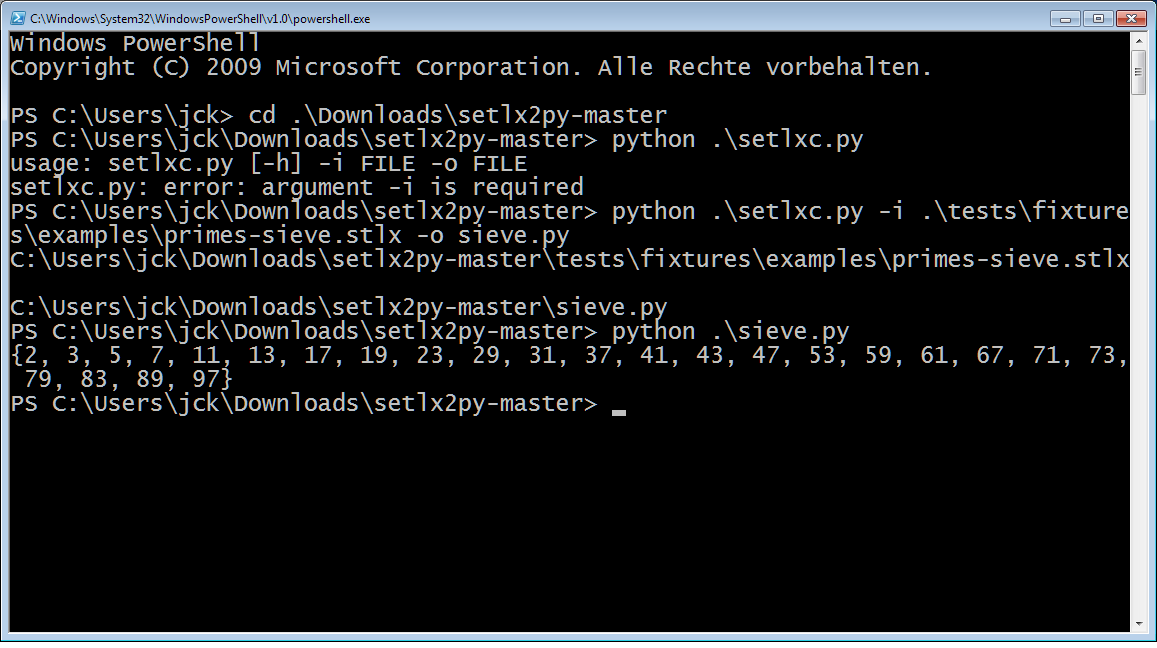
\includegraphics[width=0.8\textwidth]{img/sieve.png}
    \caption{Using setlx2py to compile SetlX and running the generated Python}
    \label{fig:use-sieve}
\end{figure}